 \documentclass[thesis-solanki.tex]{subfiles}



\ifMain
\externaldocument{thesis-solanki}
\fi
\begin{document}

%----------------------------------------------------------------------------
\chapter{Work Completed}\label{chap:workCompleted}
%----------------------------------------------------------------------------


\section{What is this chapter about}

-----------------------------------------------------------------------------


\section{What we are doing}
A partial implementation of the logic programming language \progLang{Prolog} is provided by the library \texttt{prolog-0.2.0.1}. One of the 
objectives is to implement monadic unification using the library \cite{unification-fd-lib}. 


\section{Unifiable Data Structures}
For a data type to be Unifiable, it must have instances of Functor, Foldable and Traversable.
The interaction between different classes is depicted in Figure \ref{fig:Functor Hierarchy Redux}.

\begin{figure}[th]
\centering
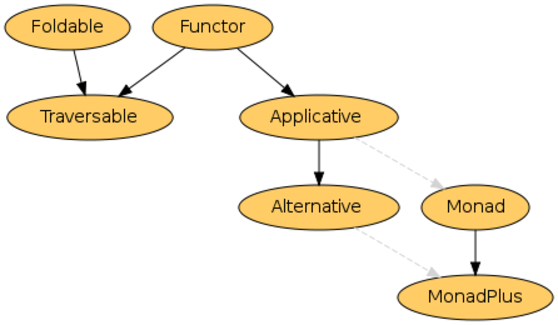
\includegraphics[scale = 0.7]{FunctorHierarchy.png}
\caption{Functor Hierarchy \cite{website:foldablenadtraversable}
(This is also Figure~\ref{fig:Functor Hierarchy}, repeated here for convenience)}
\label{fig:Functor Hierarchy Redux}
\end{figure}  

The Functor class provides the \texttt{fmap} function which applies a particular operation to each element in the given data structure. The Foldable class \textit{folds} the data structure by recursively applying the operation to each element and 

\section{Why \texttt{Fix} is necessary?}
Since \progLang{Haskell} is a lazy language it can work with infinite data structures. \textit{Type Synonyms} in \progLang{Haskell} cannot be self 
referential.


 

In our case consider the following example,

\begin{minted}{haskell}
-- The Prolog Syntax
type Atom = String
data VariableName = VariableName Int String  deriving (Show,Eq,Ord)
data FlatTerm a = 
		 Struct Atom [a]
	|	Var VariableName
	|	Wildcard
	|	Cut Int deriving (Show,Eq,Ord)
\end{minted} 
 
A \texttt{FlatTerm} can be of infinite depth which due to the reason stated above cannot be accounted for during application function. The resulting type signature would be of the form,

\mint{haskell}|FlatTerm (FlatTerm (FlatTerm (FlatTerm (.....))))|

Enter the \texttt{Fix} same as the function as a data type. The above would be simply reduced to,

\mint{haskell}|Fix FlatTerm|   

resulting in the \progLang{Prolog} Data Type
\mint{haskell}|data Prolog = P (Fix FlatTerm) deriving (Show,Eq,Ord)|

\section{Dr. Casperson's Explanation}

A recursive data type in \progLang{Haskell} is where one value of some type contains values of that type, which in turn contain more values of the same type 
and so on. Consider the following example.

\begin{minted}{haskell}
data Tree = Leaf Int | Node Int (Tree) (Tree)
\end{minted} 

A sample \texttt{Tree} would be,

\mint{haskell}|(Node 0 (Leaf 1) (Node 2 (Leaf 3) (Leaf 4)))|

The above structure can be infinitely deep since \progLang{Haskell} is a \textit{lazy} programming language. But working with an infinitely deep / nested 
structure is not possible and will result in a \textit{occurs check} error. This is because writing a type signature for a function to deal with such a
parameter is not possible. One option would be to \textit{flatten} the data type by the introduction of a type variable. Consider the following,

\begin{minted}{haskell}
data FlatTree a = Leaf Int | Node Int a a
\end{minted}  

A sample \texttt{FlatTerm} would be similar to \texttt{Tree}. 

The \texttt{FlatTree} is recursive but does not reference itself. But it too can be infinitely deep and hence writing a function to work on the structure
is not possible.  

\section{The other fix}

The \texttt{fix} function in the \texttt{Control.Monad.Fix} module allows for the definition of recursive functions in \progLang{Haskell}. Consider the 
following scenario,

\begin{minted}{haskell}
fix :: (a -> a) -> a
\end{minted}
The above function results in an infinite application stream,

\begin{minted}{haskell}
f s : f (f (f (... )))
\end{minted} 

A fixed point of a function f is a value a such that f a == a. This is where the name of fix comes from: it finds the least-defined fixed 
point of a function.

\section{The Fix we use}
Fix-point type allows to define generic recursion schemes \cite{data-fix-lib}.
\cite{website:understandingalgebrasfpcomplete}
\begin{description}
\item[What is Algebra]
Naively speaking algebra gives us the ability to perform calculations with numbers and symbols.

\item[What can algebra do]
The ability to form and evaluate expressions.

\item[How to generate expressions]
Using grammars, for example
\begin{minted}[linenos]{haskell}
data Expr = Const Int
          | Add Expr Expr
          | Mul Expr Expr
\end{minted}

\item[How to uncover primitives from a recursive type]
Make it non-recursive by defining a type function, otherwise known as type constructor,
\begin{minted}[linenos]{haskell}
ExprF a = Const Int
        | Add a a
        | Mul a a
\end{minted}

\item[How to create a nested structure from the above]
The fractally recursive structure of Expr can be generated by repeatedly applying ExprF to itself.
\begin{minted}[linenos]{haskell}
(ExprF (ExprF (ExprF a)))
\end{minted}

\item[How to generate really deep expressions]
Keep on applying \mint{haskell}|ExprF|

\item[Is there a better way]
After infinitely many iterations we should get to a fix point where further iterations make no difference. It means that applying one more 
ExprF would not change anything -- a fix point does not move under ExprF. It's like adding one to infinity: you get back infinity.   

\item[How do that in \progLang{Haskell}]
In \progLang{Haskell}, we can express the fix point of a type constructor f as a type:

\begin{minted}[linenos]{haskell}
newtype Fix f = f (Fix f)
\end{minted}
With that, we can redefine Expr as a fixed point of ExprF:
\begin{minted}[linenos]{haskell}
type Expr = Fix ExprF
\end{minted}

\item[Any other benefits]
Writing functions is simpler. You can have the terms of all depths encapsulated under the same type, i.e.
\mint{haskell}|Fix ExprF|
So rather than writing separate functions for,
\begin{minted}[linenos]{haskell}
(ExprF a)

(ExprF (ExprF a))

(ExprF (ExprF (ExprF a)))

(ExprF (ExprF (ExprF ....)))
\end{minted}

We write a function from,
\mint{haskell}|func :: Fix ExprF -> Fix ExprF|



\begin{comment}
\item[what and how to evaluate expressions]
Evaluation is a recipe for extracting a single value from an expression. 
\begin{minted}[linenos]{haskell}
instance Functor ExprF where
    fmap eval (Const i) = Const i
    fmap eval (left `Add` right) = (eval left) `Add` (eval right)
    fmap eval (left `Mul` right) = (eval left) `Mul` (eval right)
\end{minted}

We \yyy{"}{``}map\yyy{"}{''} the \yyy{"}{``}\markWord{eval}\yyy{"}{''} through our \markWord{ExpF} term for example,
\begin{minted}[linenos]{haskell}
alg :: ExprF Int -> Int
alg (Const i)   = i
alg (x `Add` y) = x + y
alg (x `Mul` y) = x * y
\end{minted}
\end{comment}

\end{description}

\begin{comment}
\begin{minted}[linenos]{haskell}
 Fix f = f (Fix f)
\end{minted}
The Essence of Algebra
There are two really essential aspects of an algebra:

The ability to form expressions and
The ability to evaluate these expressions
The Essence of Expression

The standard way of generating expressions is to use grammars. Here's an example of a grammar in \progLang{Haskell}:

\begin{minted}[linenos]{haskell}
data Expr = Const Int
          | Add Expr Expr
          | Mul Expr Expr
\end{minted}

Like most non-trivial grammars, this one is defined recursively. You may think of Expr as a self-similar fractal. An Expr, as a type, contains not only Const Int, but also Add and Mult, 
which inside contain Exprs, and so on. It's trees all the way down.

But recursion can be abstracted away to uncover the real primitives behind expressions. The trick is to define a non-recursive function and then find its fixed point.

Since here we are dealing with types, we have to\eref{must-have-to} define a type function, otherwise known as type
constructor.
Here's the non-recursive precursor of our grammar (later you'll see that the F in ExprF stands for functor):

\begin{minted}[linenos]{haskell}
ExprF a = Const Int
        | Add a a
        | Mul a a
\end{minted}


The fractally recursive structure of Expr can be generated by repeatedly applying ExprF to itself, as in ExprF (ExprF (ExprF a))), etc. The more times we apply it, the deeper trees we can 
generate. After infinitely many iterations we should get to a fix point where further iterations make no difference. It means that applying one more ExprF would't change anything -- a fix 
point doesn't move under ExprF. It's like adding one to infinity: you get back infinity.

In \progLang{Haskell}, we can express the fix point of a type constructor f as a type:

More stuff that I did not understand well can be found here,
\cite{website:understandingalgebrasfpcomplete}
\end{comment}

\clearpage

\section{Opening up or Extending language Explanation using Box Analogy}

This section will describe what it means to \textbf{\yyy{"}{``}open up or extend a language\yyy{"}{''}}. 

\begin{enumerate}
\item Let us start with a sample language with a recursive abstract syntax,
\begin{minted}[linenos]{haskell}
type Atom         	= String

data VariableName 	= VariableName Int String
      deriving (Eq, Data, Typeable, Ord)

data Term 			= Struct Atom [Term]
          			| Var VariableName
          			| Wildcard  
          			| Cut Int
      deriving (Eq, Data, Typeable)
\end{minted}

The above language represent a stripped down version of \progLang{Prolog} from \cite{prolog-lib}. The pool of the expressions that can
be generated from \textit{Term} are restricted to the constructors,   

\begin{minted}[linenos]{haskell}
Struct "hello" [Struct "a" []] 	-- hello(a).
Var (VariableName 125 "X")	-- X = 125.
Wildcard	-- _.
Cut 0	-- !.
\end{minted}

It does not allow the ability to have a \textbf{"typed"} \textit{Term}, for example a \textit{Term} of type \textit{int or string} and
so on.


\item So we \textbf{flatten} the language by introducing a type variable,

\begin{minted}[linenos]{haskell}

type Atom = String

data VariableName = VariableName Int String  deriving (Show, Eq, Ord)

data FlatTerm a = 
		Struct Atom [a]
	| Var VariableName
	| Wildcard
	| Cut Int deriving (Show, Eq, Ord)

\end{minted}

The above language can be of any type \textit{a}. A more accurate way of saying it would be that \textit{a} can be a \textit{kind} in 
\progLang{Haskell}. 

In type theory, a kind is the type of a type constructor or, less commonly, the type of a higher-order type operator. A kind system is 
essentially a simply typed lambda calculus 'one level up,' endowed with a primitive type, denoted * and called 'type,' which is the kind of 
any (monomorphic) data type for example \cite{website:kindhaskellwiki},

\begin{minted}[linenos]{haskell}
Int :: *
Maybe :: * -> *
Maybe Bool :: *
a -> a :: *
[] :: * -> *
(->) :: * -> * -> *
\end{minted}  

Simply speaking the \textit{a} can be changed.  

\item It gives the language the capability to be expanded. Adding some functionality to the original language could be done in a no.of
ways 
\begin{enumerate}
\item Manually modifying the structure of the language,
\begin{minted}[linenos]{haskell}
type Atom         	= String

data VariableName 	= VariableName Int String
      deriving (Eq, Data, Typeable, Ord)

data Term 			= Struct Atom [Term]
          			| Var VariableName
          			| Wildcard  
          			| Cut Int
          			| New_Constructor_1 .........
          			| New_Constructor_2 .........
      deriving (Eq, Data, Typeable)
      
\end{minted}

This would then trigger a ripple effect thorughout the architecture because accomodations need to be made for the new functionality.

\item The other option would be to \textit{functorize} language like we did by adding a type variable which can be used to plug something that provides the functionality into the language.
Consider the following example,

\begin{minted}[linenos]{haskell}
data Box f = Abox | T f (Box f) deriving (.........)
\end{minted}

then something like,
\begin{minted}[linenos]{haskell}
T (Struct 'atom' [Abox, T (Cut 0)])
\end{minted}
   
is possible. Since we needed the fixed point of the language we used \textit{Fix} but generically one could add multiple custom 
functionality.  

\end{enumerate}  


\item If we have a grammar that support an expressions like,


\begin{math}
x \cdot y + x \cdot z
\end{math} 

Once the language is 'functorized' one can add quantifiers and logic to the language to do something like,


\begin{align}
  \forall x \forall y & \forall z & x \cdot y + x \cdot z \\
  = & x \cdot (y + z)	
\end{align}

\item Multiple modifications

\item As is with the original language it can be wrapped with multiple other data structures,

\begin{minted}[linenos]{haskell}
Just (Strcut ......) -- A Maybe Term
[Cut 0]				-- A List of Terms
\end{minted} 
and so on. But the core expression can only be of type \textit{Term}. 

Whereas a \textit{FlatTerm} exspression can not only have an outer wrapper but also its type is 'open'.   



\end{enumerate}



\section{Chapter Recapitulation}

\ifMain
\begin{scope}
  \nolinenumbers
  \enotesize
  \par
  \begin{singlespace}
  \setlength{\parskip}{12pt plus 2pt minus 1pt}
  \theendnotes
  \par
  \end{singlespace}
\end{scope}
\unbcbibliography{bibliography}
\fi

\end{document}
